\documentclass[tikz,border=10pt]{standalone}
% Figure: D at origin, scale s = 0.011713 cm/px, y flipped
\begin{document}
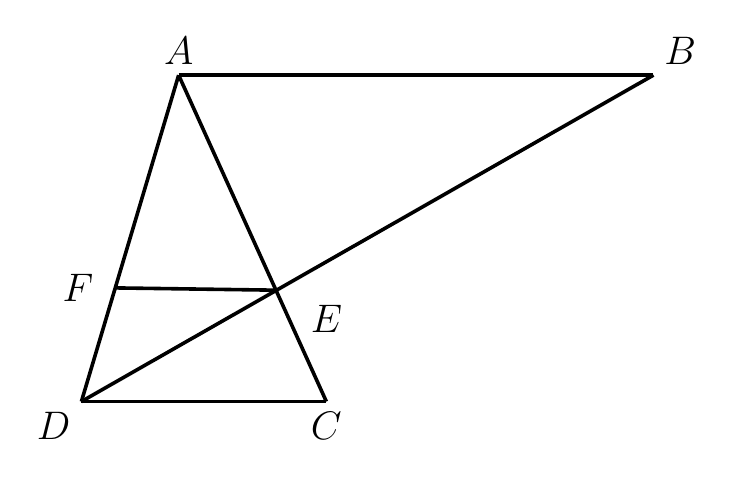
\begin{tikzpicture}[line width=1.3pt, line join=round]

  % Named coordinates (converted from pixels)
  \coordinate (A) at (1.235,4.145);
  \coordinate (B) at (7.265,4.145);
  \coordinate (C) at (3.111,0);
  \coordinate (D) at (0,0);
  \coordinate (E) at (2.474,1.414);
  \coordinate (F) at (0.431,1.443);

  % Segments
  \draw (A) -- (B);      % top horizontal AB
  \draw (A) -- (D);      % AD
  \draw (A) -- (C);      % AC
  \draw (D) -- (C);      % bottom DC
  \draw (B) -- (D);      % long BD through E
  \draw (F) -- (E);      % horizontal FE, stops exactly at E

  % Labels
  \node[above] at (A) {\fontsize{13.5}{16.2}\selectfont $A$};
  \node[above right] at (B) {\fontsize{13.5}{16.2}\selectfont $B$};
  \node[below] at (C) {\fontsize{13.5}{16.2}\selectfont $C$};
  \node[below left] at (D) {\fontsize{13.5}{16.2}\selectfont $D$};
  % E: placed south-east, clear of BD (up-right) and AC (steep, down-right)
  \node[anchor=north west, xshift=0.3cm, yshift=-0.05cm] at (E) {\fontsize{13.5}{16.2}\selectfont $E$};
  % F: west of F, shifted left ~4pt so it clears AD
  \node[left, xshift=-4pt] at (F) {\fontsize{13.5}{16.2}\selectfont $F$};

\end{tikzpicture}
\end{document}